% !TEX TS-program = pdflatex
% !TEX encoding = UTF-8 Unicode

% This is a simple template for a LaTeX document using the "article" class.
% See "book", "report", "letter" for other types of document.

\documentclass[11pt]{article} % use larger type; default would be 10pt


\usepackage{ulem}
\newcommand\NoIndent[1]{%
  \par\vbox{\parbox[t]{\linewidth}{#1}}%
}


\usepackage[utf8]{inputenc} % set input encoding (not needed with XeLaTeX)

%%% Examples of Article customizations
% These packages are optional, depending whether you want the features they provide.
% See the LaTeX Companion or other references for full information.

%%% PAGE DIMENSIONS
\usepackage{geometry} % to change the page dimensions
\geometry{a4paper} % or letterpaper (US) or a5paper or....
% \geometry{margin=2in} % for example, change the margins to 2 inches all round
% \geometry{landscape} % set up the page for landscape
%   read geometry.pdf for detailed page layout information

\usepackage{graphicx} % support the \includegraphics command and options

% \usepackage[parfill]{parskip} % Activate to begin paragraphs with an empty line rather than an indent

%%% PACKAGES
\usepackage{booktabs} % for much better looking tables
\usepackage{array} % for better arrays (eg matrices) in maths
\usepackage{paralist} % very flexible & customisable lists (eg. enumerate/itemize, etc.)
\usepackage{verbatim} % adds environment for commenting out blocks of text & for better verbatim
\usepackage{subfig} % make it possible to include more than one captioned figure/table in a single float
% These packages are all incorporated in the memoir class to one degree or another...

%%% HEADERS & FOOTERS
\usepackage{fancyhdr} % This should be set AFTER setting up the page geometry
\pagestyle{fancy} % options: empty , plain , fancy
\renewcommand{\headrulewidth}{0pt} % customise the layout...
\lhead{}\chead{}\rhead{}
\lfoot{}\cfoot{\thepage}\rfoot{}

%%% SECTION TITLE APPEARANCE
\usepackage{sectsty}
\allsectionsfont{\sffamily\mdseries\upshape} % (See the fntguide.pdf for font help)
% (This matches ConTeXt defaults)

%%% ToC (table of contents) APPEARANCE
\usepackage[nottoc,notlof,notlot]{tocbibind} % Put the bibliography in the ToC
\usepackage[titles,subfigure]{tocloft} % Alter the style of the Table of Contents
\renewcommand{\cftsecfont}{\rmfamily\mdseries\upshape}
\renewcommand{\cftsecpagefont}{\rmfamily\mdseries\upshape} % No bold!

%%% END Article customizations


\usepackage{verbatim}
\usepackage{amsmath}


\title{Work Log for December}
\author{Logan Brown}
%\date{} % Activate to display a given date or no date (if empty),
         % otherwise the current date is printed 

\begin{document}
\maketitle
\tableofcontents

\newpage


\section{Goals for the Month}
As of December 1st.
%Paste output from writeGoals
\begin{enumerate}
\item Verify logMu Flip by larger runs
\item Investigate Problematic Codons
\item Is it worth it to adjust Delta a\_12?
\item Fix Names
\item Move to Newton?
\end{enumerate}

\section{Progress/Notes}

\subsection{Verify logMu Flip by larger runs}
Verified!

Doing a run of 6000 steps is definitely long enough, especially if you look at the log likelihood trace (not included for brevity). The logMu looks a bit more convincing, and also,it improve the behavior of the hyperparameters like $\sigma_\epsilon$ and $\sigma_\phi$. For the first 300 or so samples, the model has to fit to the negative $log(\mu)$ value. To its credit, the model does so, but that's not good.

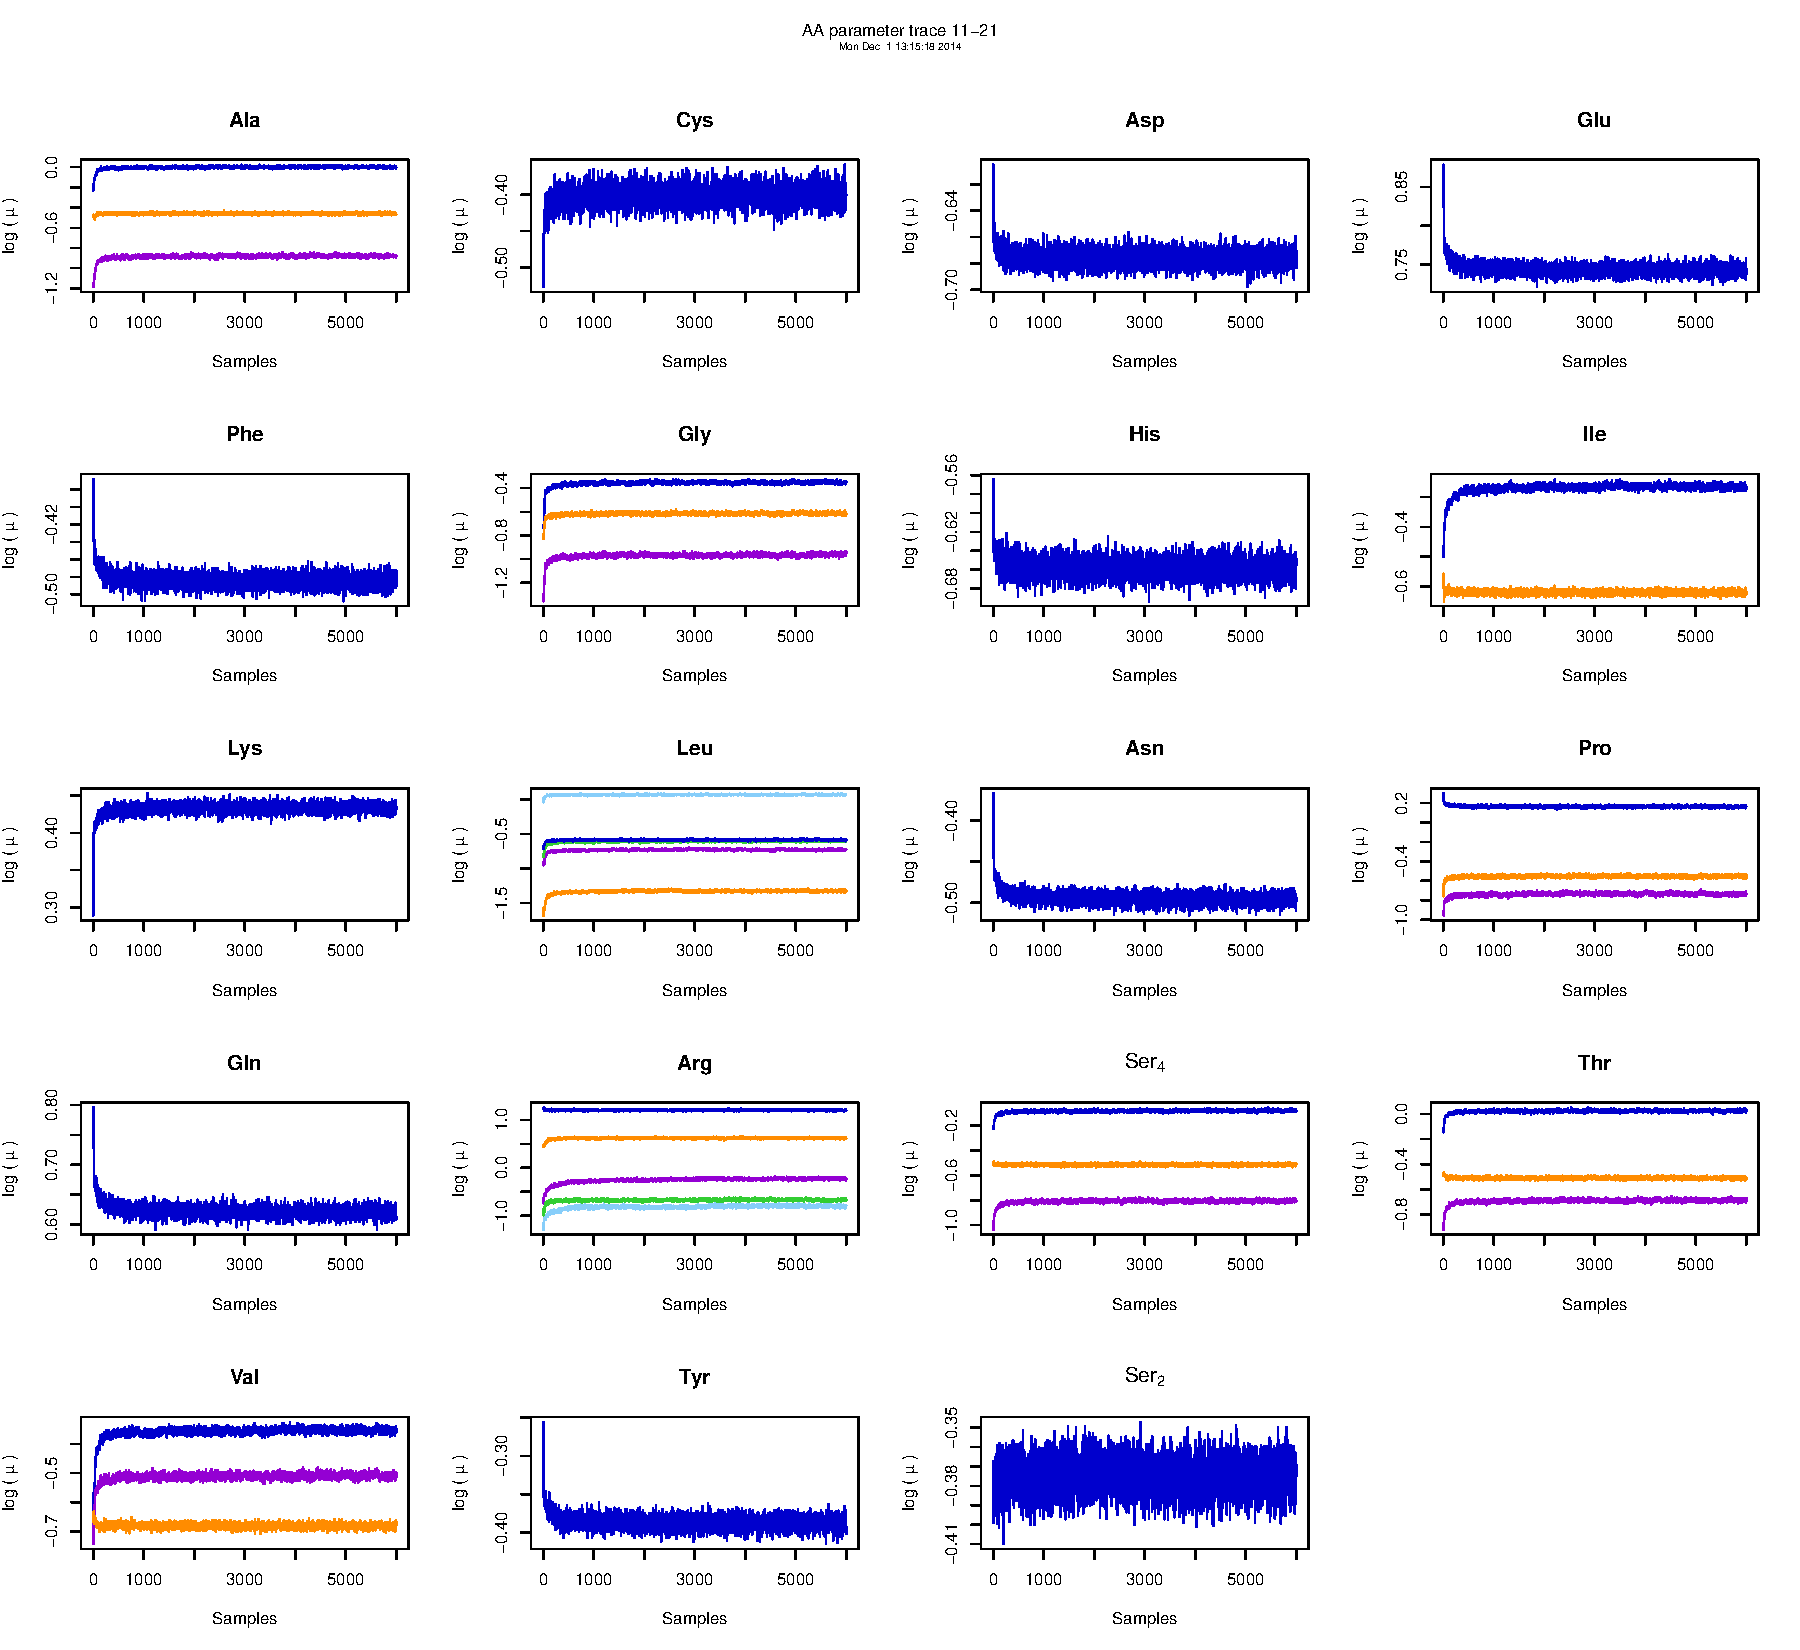
\includepdf[pages={1}]{data/11-21-logmu-6000-1a2-Mflip.pdf}
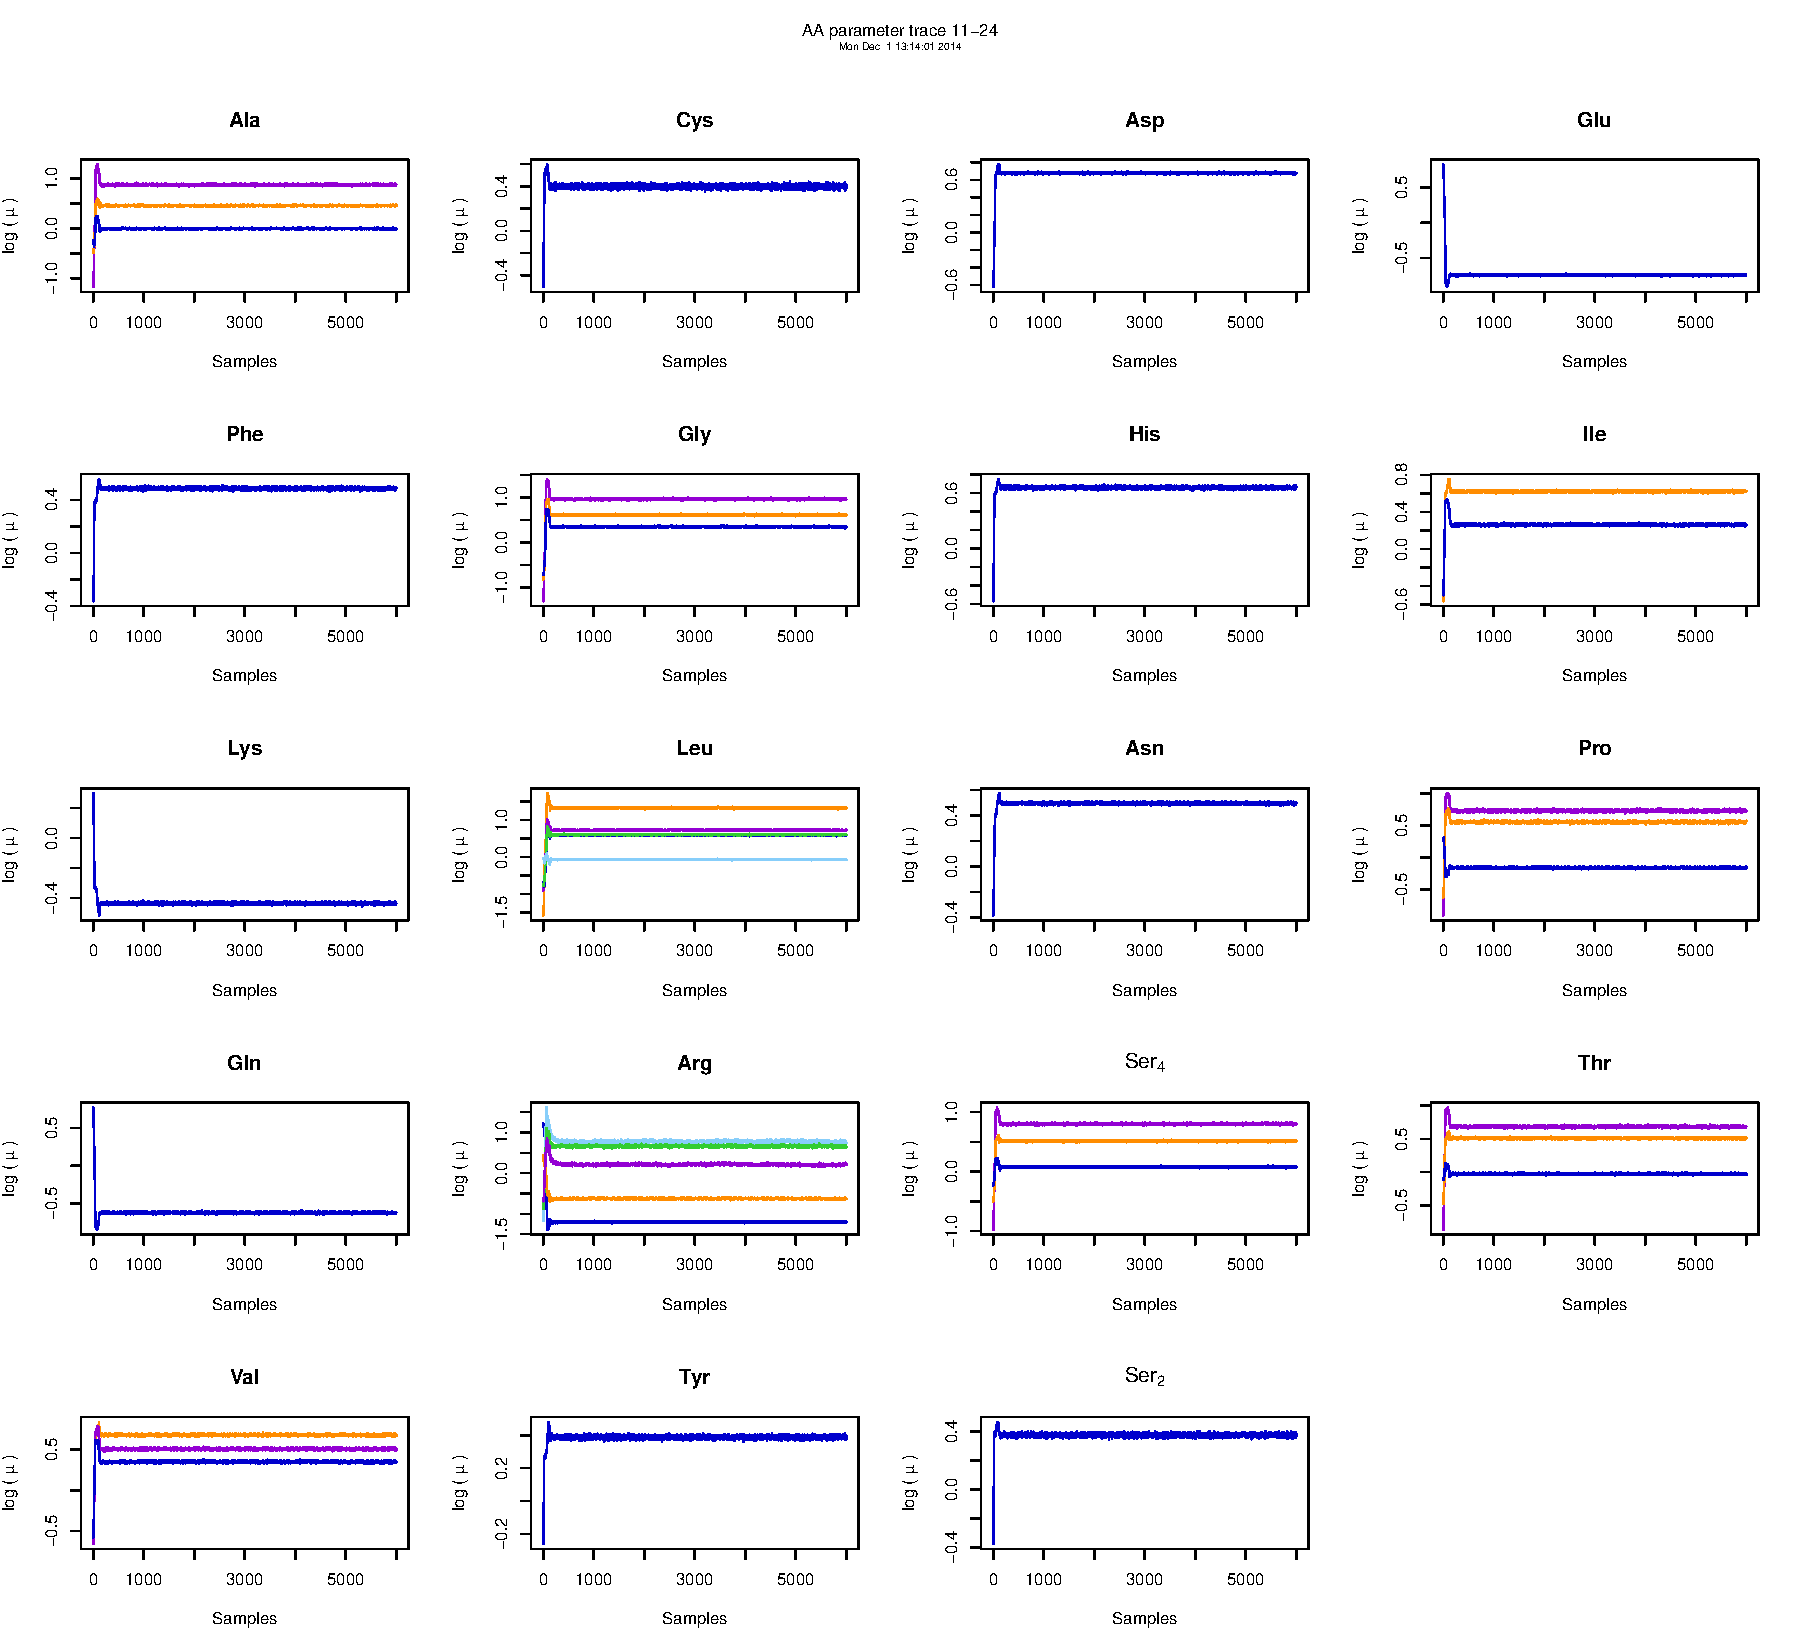
\includepdf[pages={1}]{data/11-24-logmu-6000-4a2-noMflip.pdf}

\begin{figure}[h!]
\caption{The left figure is a run before the logMu flip. The right is after. You can see that before fixing the logMu flip, the hyperparameters see a huge spike early on, which quickly subsides, while on the right, you simply see them increase at the beginning as the model begins to fit, then fall off slowly as the model converges.}
\begin{tabular}{c|c}
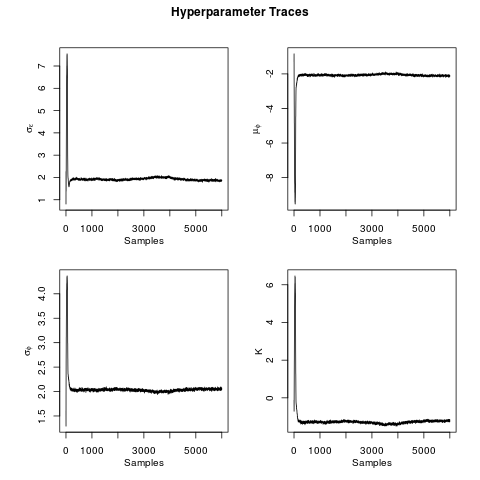
\includegraphics[width=0.48\textwidth]{data/11-24-hyperparameters-6000-4a2-noMflip.png}
&
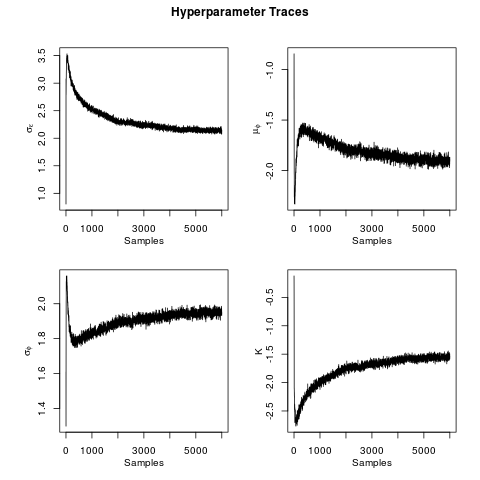
\includegraphics[width=0.48\textwidth]{data/11-21-hyperparameters-6000-1a2-Mflip.png}
\end{tabular}


\end{figure}


\subsection{Investigate Problematic Codons}

One thing we were interested in looking at was comparing the problematic $\omega$ values to their problematic log$\mu$ values. Here's a mapping!

Green Square: Leucine CTT

Yellow Diamond: Proline CCG

Blue Up Arrow: Arginine CGA

Purple Down Arrow: Arginine CCG

As we anticipated, higher nonsense error rates lead to lower mutation rates, and lower nonsense error rates lead to higher mutation rates. The magnitude is a bit off, the lowest mutation does not cause the highest nonsense errors.

This was also reproduced when using different sections of the Yeast Genome. Here are 3 distinct sections of preston's simulated yeast (they share no genes in common) that produce similar results.

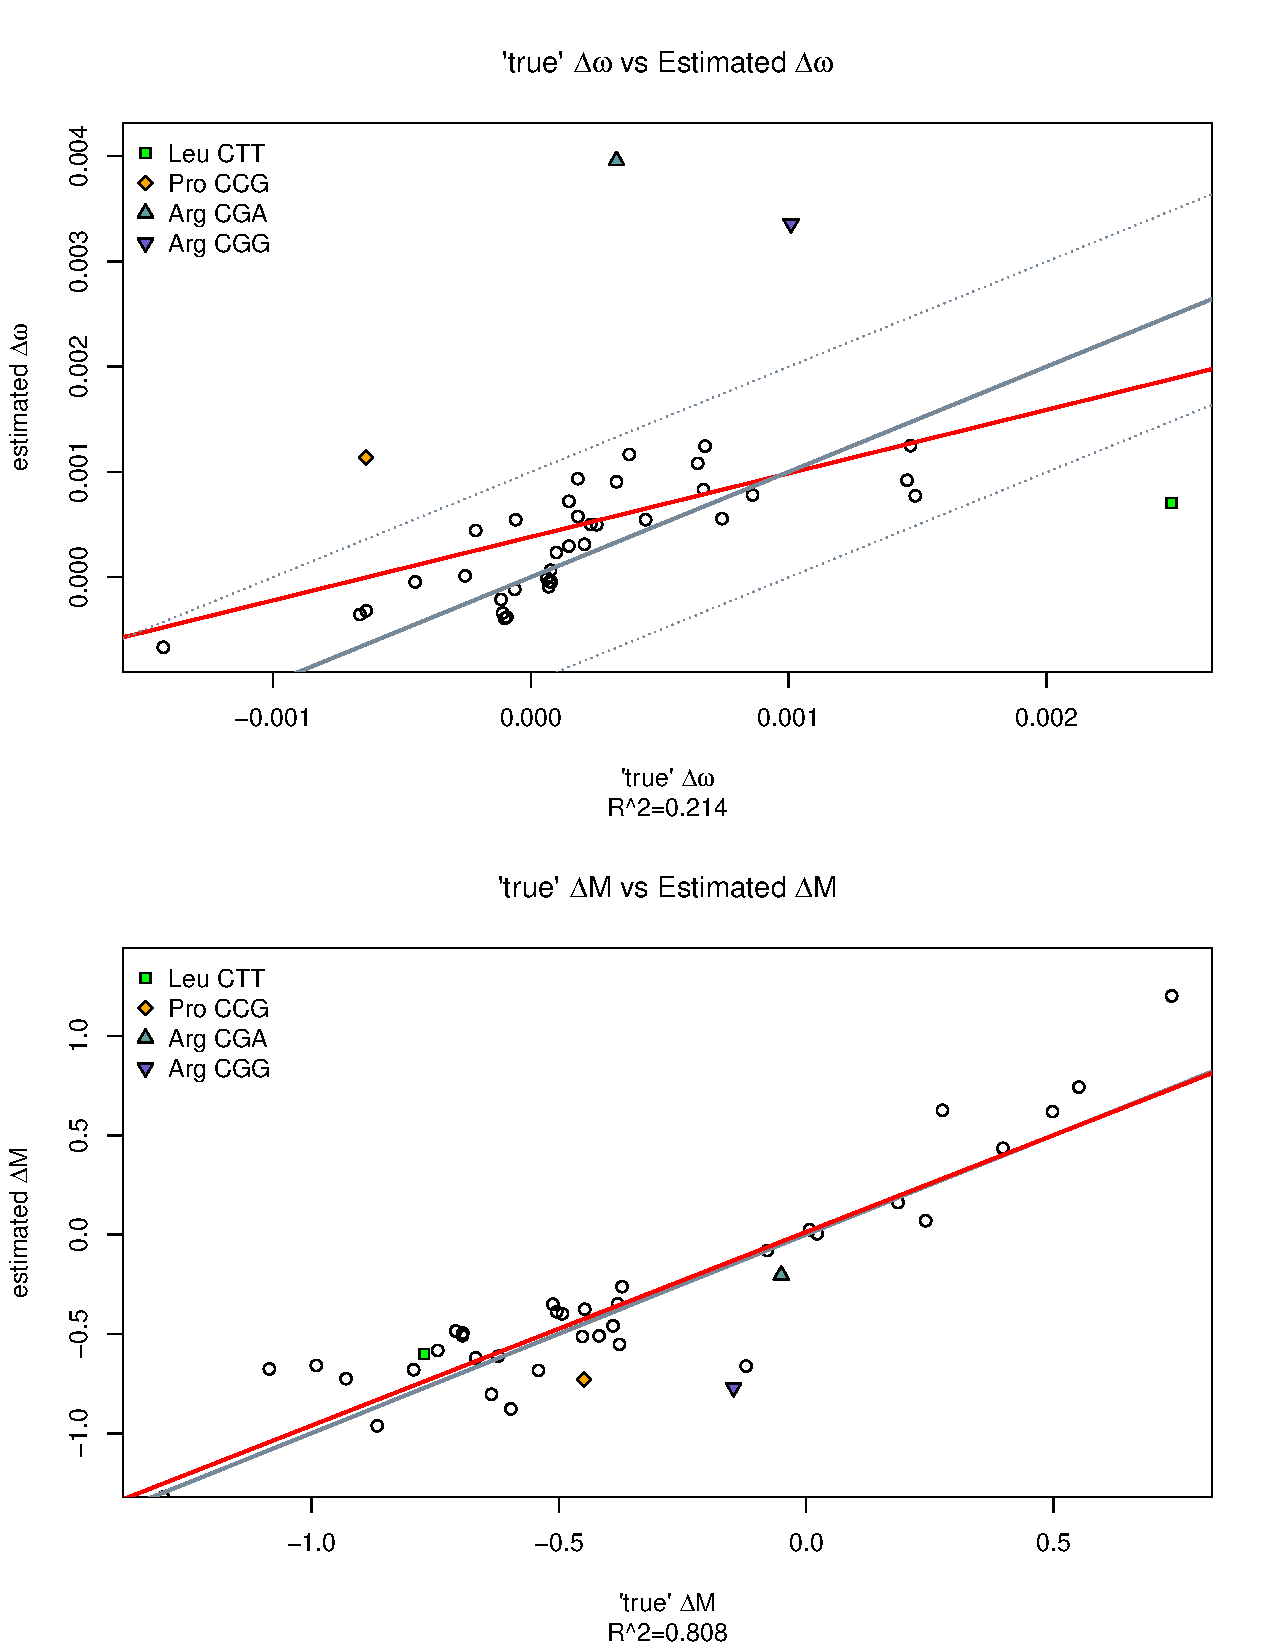
\includepdf[pages={1}]{data/errormap.pdf}

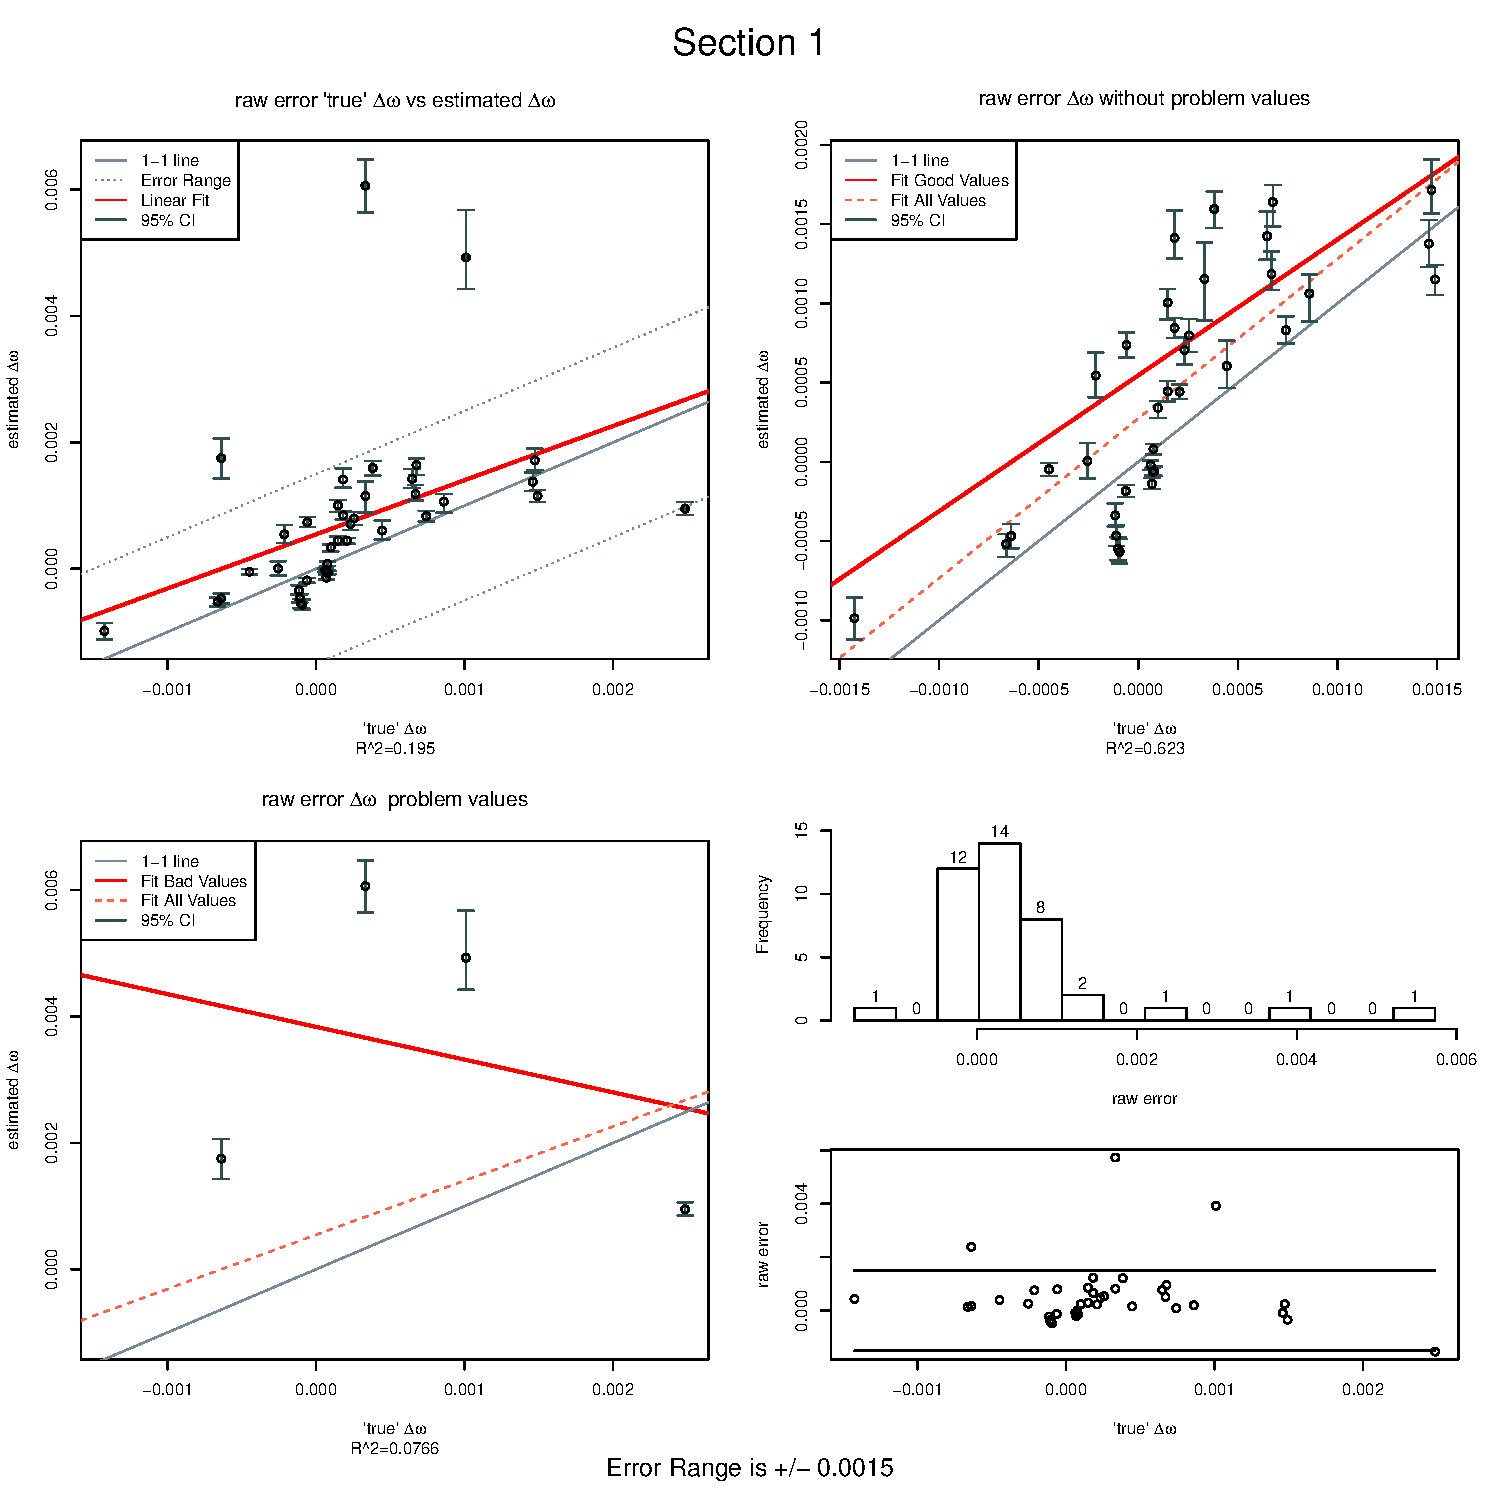
\includepdf[pages={1-3}]{data/sectionedOmegaStudy.pdf}


\subsection{Generate a new Genome}

DONE.

\sout{By modifying preston's old code, I was able to create two new simulated genomes that used the same inputs as Preston's yeast, but are new and different.}

\subsubsection{Fix the Code}

Preston's code had a problem where the simulation was only updating the c\_index, but was never actually updating the codons used. Then, when writing the genome, it wrote out the codons used. The result was that the output was identical to the input, even when the input was nonsense.

My fix uses a for loop to generate a character array of the correct codons, which it then converts to a factor and uses to replace the one in gene.list\$gene.dat\$codon

If I work on this again in the future, I want to change the code so that the stop codon is no longer given index 99, so that I can actually mutate and translate the stop codon over

These changes are also being committed to github in a repository forked from clandere.

\subsubsection{Use same inputs as Preston}

\subsubsection{Use reference codons from preston, and delta omega from run results}

\subsection{Is it worth it to adjust Delta a\_12?}

\subsection{Fix Names}

May have fixed the names by doing the following in cedric.mapBMatNames.r

\begin{verbatim}
 if(model == "roc"){
\end{verbatim}

to

\begin{verbatim}
 if(model == "roc" || model == "nsef"){
\end{verbatim}

Luckily, the functions already exist to get the coefficients for the ROC, NSE and ROCandNSE models, so I didn't have to change anything (so far)

\subsection{Speed up C code}

I made the following change in stable\_exp.c

\begin{verbatim}
	for(k = 0; k < *K; k++){
	       a_Z_normalized[k] -= max_exp;
	}

	for(k = 0; k < *K; k++){
	        a_Z_normalized[k] = exp(a_Z_normalized[k]);
	        *total_sum += a_Z_normalized[k];
	}
\end{verbatim}

to

\begin{verbatim}
	for(k = 0; k < *K; k++){
	        a_Z_normalized[k] = exp(a_Z_normalized[k] - max_exp);
	        *total_sum += a_Z_normalized[k];
	}
\end{verbatim}

The actual time on these operations is quite small, but since it has to happen \sout{hundreds of thousands of times} 2.8 million times for each step, it may actually cause an impact. Who knows?

The actual time difference is hard to measure, apparently.

I can measure it in microseconds, but the difference appears to be less than a microsecond, because it tends to come out as either a difference of 1 or 0 microseconds. There is a strange error where in the old version, the difference is 20 or more microseconds. If we give those credit, I seem to have reduced the run by between 1.4 and 5 microseconds. This doesn't sound like a lot, however, this code gets run millions of times for each cubfits run. Simulated yeast has 2.8 million codons, which means that this reduction would be 3.9 seconds less per proposal. Assuming 50,000 proposal states, that's 54 hours less. Which is quite unbelievable, since the runs don't even go that long.

So, assuming distances greater than about 5 microseconds are unbelievable, we can extrapolate what the actual change is. By averaging the values less than 5 microseconds (mostly 0s and 1s), we can guess how much the change actually is in microseconds. Using conservative estimates, it looks to be about .05 microseconds. Assuming 2.8 million codons and 50,000 MCMC proposed states, that's still a difference of 2 hours per run. The actual difference could be closer to .1 microseconds, which would be 4 hours per run.

\subsection{Move to Newton?}


\section{Goals for next Month}
\begin{enumerate}
\item Future Goal
\end{enumerate}


\end{document} %End of day document, REMOVE
